\documentclass{llncs} %
\bibliographystyle{splncs}
\usepackage{url}
\usepackage{graphicx}

\newcommand{\source}[1]{\hfill Source: {#1} }

\begin{document}

\title{Supporting Meditative Awareness through Neurofeedback Wearables}
\author{Vincenzo Pace}
\institute{Karlruhe Institute of Technology, Karlsruhe, Germany}
\maketitle
\newpage
\section{Introduction}
Adoption and functionality of wearable devices are increasing and expected to continue to do so \cite{Patel}. In the west, meditation is accepted more widely as a means of health improvement \cite{Tang:et al}.
Consumer EEG devices and freely available EEG/ERP databases \cite{ucsd} offer a chance to use algorithms to analyze a user's meditation experience and provide feedback for improvement.
This work presents the current state of art of consumer EEG devices, the signals involved in meditation and the possibility for usage of such devices for meditation training.
In the end, three popular EEG headsets will be compared and evaluated.
\subsection{EEG}
EEG stands for electroencephalography and is a process to record the electrical activity in the brain. The measured signal are voltage changes in and between neurons. EEG can only measure measure signal in the outer regions of the brain \cite{Sitaram}.
The brains signal is in the order of mikrovolt \cite{Berger}.  For measurement, EEG electrodes are placed on the test subjects scalp. In Research, up to 256 electrodes are used \cite{Seeck}, while consumer grade devices use around 10\% of this. \cite{Maskeliunas}
The electrical signal is measured as frequencies and goes through an EEG ampflifier. These get passed to a Fast Fourier Transformation (FTT) or wavelet transformation \cite{Akin} to produce distinct waves, which are then categorized according to known patterns \cite{Shaker}.
Brain waves of individuals can be compared to aggravated data of many test subjects, to search for disorders \cite{Loo} or match for meditation success \cite{Tang:et al}, access to enough datapoints assumed.
There are four main brain frequencies \cite{Cahn}:
% quantitative eeg 
\begin{itemize}
    \item 
    Beta Waves (frequency range from 14 Hz to about 30 Hz), associated with intellectual activity and outwardly focused concentration
    \item 
    Alpha Waves (frequency range from 7 Hz to 13 Hz), associated with relaxation
    \item 
    Theta Waves (frequency range from 4 Hz to 7 Hz), associated with mental inefficiency \cite{Hammond}, zone between wake and sleep
    \item 
    Delta Waves (frequency range up to 4 Hz), associated with sleeping, learning disabilities \cite{Hammond}
\end{itemize}
From the data, conclusions about attention \cite{Berka}, stress \cite{Hosseini}, cognitive load \cite{Antonenko} and more are possible.
While EEG caps are usually used in research and academia \cite{Seeck}, headsets provide a reasonable solution for consumers with less complexity, but also lower precision\cite{Maskeliunas}.
For the accuracy of the measurement it is still crucial, that the sensors are correctly affixed \cite{Seeck}, so that they measure the brain regions that are involved in meditation.

EEG devices are either gel based or dry. In Research, gel electrodes are used and cost thousands of dollars, have wired signal transmission and are time consuming to setup and are uncomfortable to wear.
Consumer devices on the other hand are dry, wireless and cost only a few hundreds of dollars. \cite{Decho}
\subsection{Neurofeedback}
Neurofeedback (NFB), also called EEG biofeedback, is a therapy that was invented as a method for training brainwave patterns through operant conditioning and is known since the 1960s \cite{Hammond}. %OK like that?
It is used not only as a treatment of disorders \cite{brand:del}, but also in peak performance training \cite{Kaufman}. NFB experiments led to the deleopment of the field of brain-machine interfaces \cite{Sitaram}.
Operant conditioning is the learning process where a behavior is modified by punishment or reward \cite{Spence}. NFB never uses punishment though. In NFB, the neural activity is recorded and presented to the participant in real time, either auditory or visual.  
Usually people are not aware of their brain waves, so seeing them on a screen helps by giving you the ability to influence them. This is the operant conditioning part. In the beginning, the changes are only short-lived, but with practice can become lasting. 

\begin{figure}
    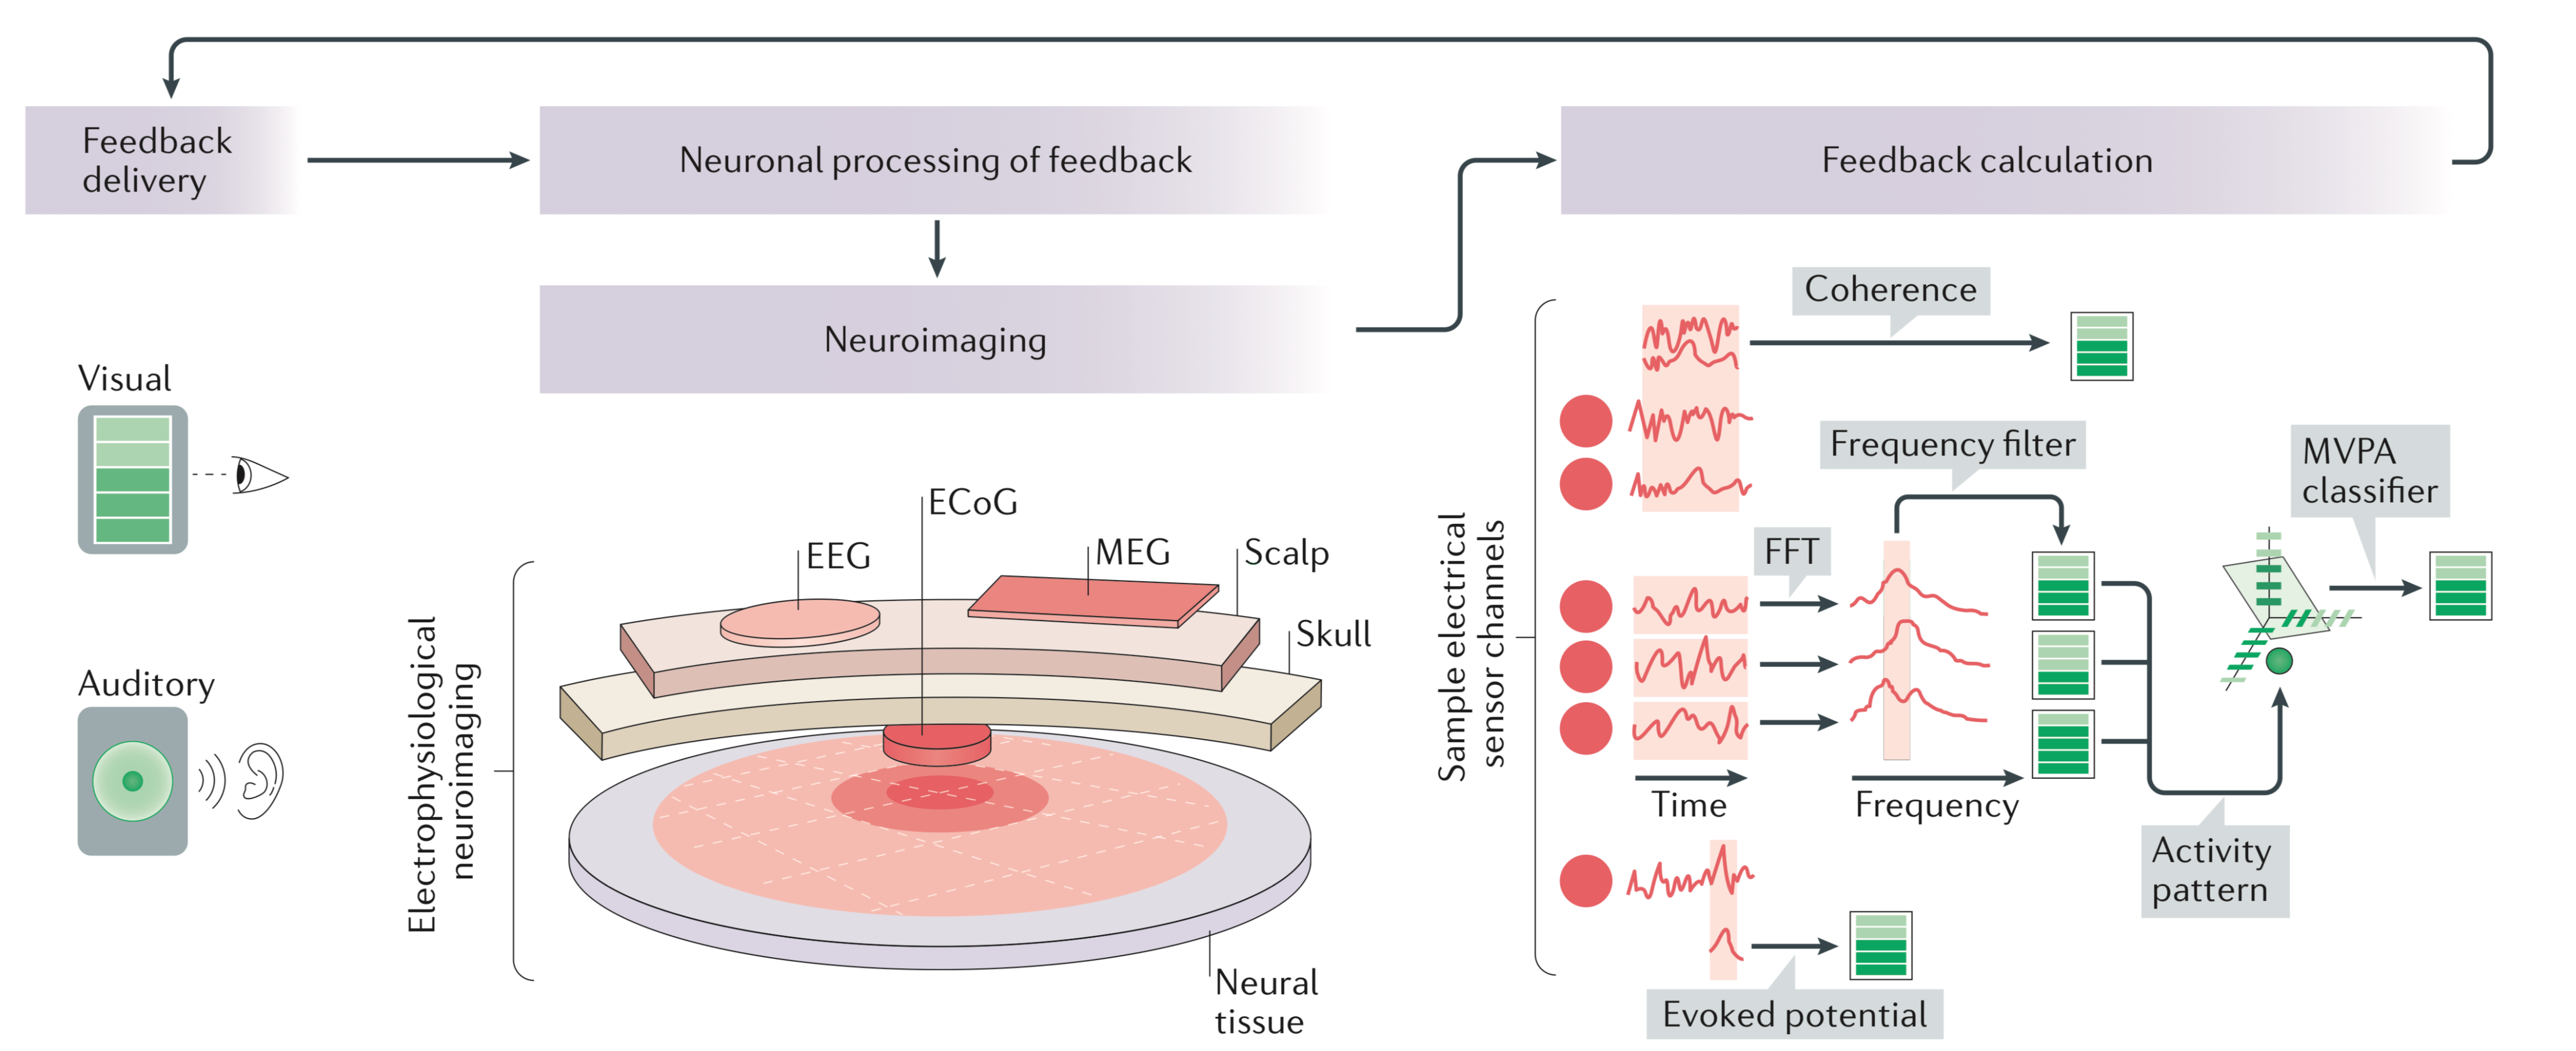
\includegraphics[width=\linewidth]{Neurofeedback.png}
    \caption{The neurofeedback process}  \label{neurofeedback}
    \source{Sitaram et al, 2016}
\end{figure}

NFB is non-invasive and is sometimes used as an alternative to medication \cite{Hammond}. Another unique kind of NFB is called LENS, where a tiny electromagnetic signal is introduced to the electrodes and transported to the brain.
However, it is not recommended to use NFB equipment without any expertise. Also, the training should be individualised to the unique brainwave patterns of each person. A physician should always be consulted first.
Otherwise, negative side effects or degradation of existing disorders are possible. Only healthy individuals should use a NFB device for meditation training on their own risk.

\subsection{Meditation}
Over the last decades, meditation has gained the interest of popular culture and the scientific community.
Documented beneficial effects range from mood improvements to structural changes \cite{Davidson} in various regions of the brain, such as the amygdala (responsible for stress and anxiety), anterior cingulate cortex, brain stem (breathing)
and the default mode network \cite{Tang:et al}.
Therefore, meditation has become part of psychiatric interventions \cite{Hoelzel}, high performance sports and personal development.
Historically, meditation stems from buddhist practices and has been part of eastern culture for centuries, though variations were also practiced by the ancient greeks \cite{Hadot:Davidson}.

Though there is not one single meditation practice, the methods are plentiful. While often associated with stillness and watching ones breath,
there are also more active forms of meditation that involve more movement. Travis and Shear categorize meditation practices into focused attention, open monitoring and automatic self-transcending.\cite{Travis} 
Since this categorization is based on different EEG patterns and would be part of the wearable device, I will follow this categorization and differentiate where appropriate.
\subsection{Awareness}
Mindfulness and awareness are two terms often mentioned in the context of meditation and there is no exact, agreed upon scientific definition to separate these two. Merriam Webster lists the two terms as synonimous and defines awareness as: "knowledge and understanding that something is happening or exists" \cite{Merriam:Webster}. 

In current research contexts, mindfulness is typically defined as nonjudgmental attention to experiences in the present moment \cite{Kabat-Zinn}.
\section{Goals}
Since the beneficial effects of meditation are so various, the goals of using a wearable device 
that provides neurofeedback to its user are inherently diverse. Machine assisted meditation could help individuals to 
improve faster, track their progresssion, analyze the state of mind and lower the entrance barrier for novel practicioners. \cite{brand:del}
All of these different features can be combined in an app targeted at consumers. 
The differences in EEG signals induced by the different meditation practices enable a categorization
and dedicated training regime to offer the device and software solution to a wider audience. \cite{Travis}
\section{Measurement Data}
\subsection{Biological Signals}
\begin{itemize}
    \item EEG
    \item brain blood flow infrared spectroscopy
    \item ECoG
    \item MEG 
    \item NIRS
    \item BOLD
    \item haemodynamics
\end{itemize}
Combination of NIRS and EEG would be optimal! There is no such device yet for consumers though.
Possible?

EEG band meditation.



\textbf{Welche (gehirn-)signale sind biologisch relevant für meditation? --> welche signale kann ich messen (insbesondere auch welche signale sind für low cost geräte geeignet: hardwarekosten, messdauer, ... )?}


\subsection{Measuring}
\textbf{welche signale bekomme ich, warum kann ich die mit so einem "billigen" gerät schon messen? wie funktioniert das?...}
\subsection{Challenges}
Such a QEEG Assesment usually takes about 1.5 hours, which is too long for a consumer.
Involuntary movement of the tongue, eyeballs, jaw and facial muscles produce noise in the milivolt range, while brain signals are on 
the order of mikrovolt. These artifacts do not only occur in consumer grade EEG devices, but also in medical grade.
These artifacts need to be filtered out to produce a reliable signal for further analysis \cite{Bashivan: et al}, which will be extremely difficult, since the device would need to know when a person moved ever so slightly \cite{Hammond}.

The time window of measurement is also crucial for the accuracy of machine learning models. \cite{Bashivan: et al}


Many learning theories and for the algorithm we need to decide which one we want to use as basis. 

However, as cognitive strategies activate a network (see below), neural specificity can be experimentally addressed using control conditions such as oppos- ing directions of regulation37, differential feedback51, inverted feedback52, sham feedback53, mental imagery without any feedback53 or feedback from a different neural substrate54. \cite{Sitaram}

Neurofeedback training may not always result in behavioural modifications. Studies in monkeys showed that the response of neurons in the motor cortex to operantly learned rewards are initially associated with active limb movements, but, as the monkey continues to activate the reward-linked neurons, the movements drop out entirely \cite{Sitaram}

EEG signal might not be enough. \cite{Travis}.

Most neurofeedback systems provide auditory or visual feedback that fully engage and demand the attention of the subject \cite{brand:del}

Subjects just learn upregulating and downregulating EEG instead of actual meditation.

Despite its promise, neurofeedback faces several chal- lenges, including the failure of some individuals to achieve self-regulation, inter-individual differences in learning capacity, uncertain long-term effects and unclear transfer benefits. Indeed, a substantial propor- tion — up to 30\% — of participants in neurofeedback and BCI studies fail to self-regulate specific brain activity even after repeated training.



It was common for inexperienced users to wear the device too low on the forehead so the electrodes were placed over a sinus cavity rather than brain. This led to weaker than expected reading for frontal signals. Users with thick hair typically had problems getting a good contact with the temporal electrodes. \cite{Bashivan: et al}

What is much less clear is whether and how meditation practices produce increased alpha beyond that obtained from reducing gen- eral arousal, which may become apparent only when fine-grained topographic mapping is combined with other neuroimaging meth- ods \cite{Cahn}

\subsection{Processing and evaluation}
\textbf{wie werden diese Signale vom gerät (hardware, software) erkannt und verarbeitet? --> wie können diese Signale für den Softwareentwickler in Anwendungen umgesetzt werden?}



In real-time analysis, the signal that is extracted from these methods is typically transformed into the frequency domain and decomposed into a specific frequency (for example, delta (0–4 Hz), theta (4–7 Hz), alpha (8–12 Hz), beta (12–30 Hz) and gamma (>30 Hz) bands) before feature extraction. Examples of feature extraction include coherence, power spectral density and their combinations for input to multivariate patterns, event-related potentials and slow cortical potentials. The signals can be processed either in sensor space (that is, individual electrodes) or source space (for example, beam formers164 or LORETA165) that enables a more accurate estimate of the activity in cortical regions that then is transformed into the feedback signal16 \cite{Sitaram}.

\textbf{Feature extraction} Independent Component Analysis, Discrete Wavelet Transform 

Preprocessing, Signal Denoising (Wavelet), FTT

We find our classification approach is able to distinguish between the baseline and meditation state on a second-by- second basis with a mean balanced success rate of 75.7\% \cite{Dixit}

EEG power spectrum analysis



\cite{Lotte}

Multivariate pattern analyses (MVPAs) was used to decode whole brain states associated with sustained atten- tion while participants performed a cognitive task. The level of difficulty of this task was automatically adjusted based on the decoded brain state to improve vigilance. \cite{Sitaram}
\section{Training procedure}
Learning to control brain activity in humans is determined by contingent feedback and reward, and potentially by ver- bal instructions and mental strategies (for example, use of imagery) that are suggested by the experimenter to the participant. \cite{Sitaram}

Assuming that reliable and repro- ducible EEG signatures are associated with specific meditation practices, we may expect that training subjects to reproduce these signatures would support and strengthen their meditation practice.
Clinical neurofeedback protocols are aim- ing toward comparing patients’ EEG with large EEG data sets from normal sub- jects in order to produce a neurofeed- back algorithm which rewards subjects (patients) whose EEG becomes closer to that of the normal population (Thornton and Carmody, 2009) \cite{brand:del}
\section{Available Devices}
In the following sections, three consumer EEG headsets will be compared. The studies used as a basis of my analysis are a few years old. In a such a fast moving field, the information might already be outdated. While one device was best a few years ago, it might not even be sold today. Thus, I try to present more general features of devices in a certain price category. While I focus on consumer grade EEG headsets, I will also look into one research grade device. What is professional performance now, will likely be achievable in consumer electronics in a few years. Thus, this can be seen as an outlook of what might be used by software engineers soon.
\subsection{Neurosky - Mindwave Mobile 2}
\subsection{InteraXon Inc. - Muse 2}
\subsection{Emotiv - Insight 5}
EMOTIV is an award-winning San Francisco based BCI company founded in 2011. They target researchers, companies and consumers with their products. Several independent papers using their products have been published. They offer an App and multiple EEG headsets. The EMOTIV Insight 5 EEG headset is their consumer device with a price of 300\$. With their software, they provide detection of facial expressions, which are important in noise detection, and mental metrics such as stress and focus. The EEG sensor uses five channels, two references above the ears and is made of a semi-dry polymer that needs to be moistened before usage. The nine axis motion sensors detect head movements. \cite{Emotiv1}


\subsection{Emotiv - EPOC+}
The EPOC internally samples at a frequency of 2048 Hz, which then gets down-sampled to 128 Hz sampling frequency per channel, and sends the data to a computer via Bluetooth. It utilizes a proprietary USB dongle to communicate using the 2.4 GHz band. Prior to use, all felt pads on top of the sensors have to be moistened with a saline solution \cite{Kushaba}
The Emotiv EPOC is a high resolution, neuro-signal acquisition and processing wireless headset that monitors 14 channels of EEG data and has a gyroscope measure for 2 dimensional control

\section{The optimal device}
However, we believe that with the development of novel approaches, such as thin tattoo-type elec- trodes, EEG recording will become practical in a much wider spectrum of real-life scenarios, and that recognizing mental states using wearables devices will become much more widespread \cite{Bashivan: et al}
\section{Conclusion}

\newpage
\begin{thebibliography}{[MT1]}
    \bibitem{brand:del}
    Tracy Brandmeyer, Arnaud Delorme,
    Meditation and neurofeedback
    Frontiers in Psychology, Article 688 (October 2013).
    \bibitem{Tang:et al}
    Tang, Yi-Yuan, Britta K. Hölzel, and Michael I. Posner. "The neuroscience of mindfulness meditation." Nature Reviews Neuroscience 16.4 (2015): 213-225.
    \bibitem{Bashivan: et al}
    Bashivan, Pouya, Irina Rish, and Steve Heisig. "Mental state recognition via wearable EEG." arXiv preprint arXiv:1602.00985 (2016).    
    \bibitem{Travis} 
    Travis, Fred, and Jonathan Shear. "Focused attention, open monitoring and automatic self-transcending: categories to organize meditations from Vedic, Buddhist and Chinese traditions." Consciousness and cognition 19.4 (2010): 1110-1118.
    \bibitem{Hoelzel}
    Hölzel, Britta K., et al. "How does mindfulness meditation work? Proposing mechanisms of action from a conceptual and neural perspective." Perspectives on psychological science 6.6 (2011): 537-559.
    \bibitem{Cahn}
    Cahn, B. Rael, and John Polich. "Meditation states and traits: EEG, ERP, and neuroimaging studies." Psychological bulletin 132.2 (2006): 180.
    \bibitem{Braboszcz}
    Braboszcz, Claire, and Arnaud Delorme. "Lost in thoughts: neural markers of low alertness during mind wandering." Neuroimage 54.4 (2011): 3040-3047.
    \bibitem{Zoefel} 
    Zoefel, Benedikt, René J. Huster, and Christoph S. Herrmann. "Neurofeedback training of the upper alpha frequency band in EEG improves cognitive performance." Neuroimage 54.2 (2011): 1427-1431.
    \bibitem{Berger}
    Berger, Hans. "Über das elektrenkephalogramm des menschen." European archives of psychiatry and clinical neuroscience 87.1 (1929): 527-570.
    \bibitem{Seeck}
    Seeck, Margitta, et al. "The standardized EEG electrode array of the IFCN." Clinical Neurophysiology 128.10 (2017): 2070-2077.
    \bibitem{Maskeliunas}
    Maskeliunas, Rytis, et al. "Consumer-grade EEG devices: are they usable for control tasks?." PeerJ 4 (2016): e1746.
    \bibitem{Surangsrirat}
    Surangsrirat, Decho, and Apichart Intarapanich. "Analysis of the meditation brainwave from consumer EEG device." SoutheastCon 2015. IEEE, 2015.
    \bibitem{Akin}
    Akin, Mehmet. "Comparison of wavelet transform and FFT methods in the analysis of EEG signals." Journal of medical systems 26.3 (2002): 241-247.
    \bibitem{Shaker}
    Shaker, Maan M. "EEG waves classifier using wavelet transform and Fourier transform." brain 2 (2006): 3.
    \bibitem{Lotte}
    Lotte, Fabien, et al. "A review of classification algorithms for EEG-based brain–computer interfaces." Journal of neural engineering 4.2 (2007): R1.
    \bibitem{Antonenko}
    Antonenko, Pavlo, et al. "Using electroencephalography to measure cognitive load." Educational Psychology Review 22.4 (2010): 425-438.
    \bibitem{Berka}
    Berka, Chris, et al. "Real-time analysis of EEG indexes of alertness, cognition, and memory acquired with a wireless EEG headset." International Journal of Human-Computer Interaction 17.2 (2004): 151-170.
    \bibitem{Hosseini}
    Hosseini, Seyyed Abed, and Mohammad Ali Khalilzadeh. "Emotional stress recognition system using EEG and psychophysiological signals: Using new labelling process of EEG signals in emotional stress state." 2010 international conference on biomedical engineering and computer science. IEEE, 2010.
    \bibitem{Loo}
    Loo SK, Barkley RA. Clinical utility of EEG in attention deficit hyperactivity disorder. Appl Neuropsychol 2005; 12(2): 64-76.
    \bibitem{Davidson}
    Davidson, Richard J., and Antoine Lutz. "Buddha's brain: Neuroplasticity and meditation [in the spotlight]." IEEE signal processing magazine 25.1 (2008): 176-174.
    \bibitem{Decho}
    Surangsrirat, Decho, and Apichart Intarapanich. "Analysis of the meditation brainwave from consumer EEG device." SoutheastCon 2015. IEEE, 2015.
    \bibitem{Hadot:Davidson}
    Hadot, Pierre; Arnold I. Davidson (1995) Philosophy as a Way of Life: Spiritual Exercises from Socrates to Foucault ISBN 0-631-18033-8 pages 83-84
    \bibitem{Patel}
    Patel, Mitesh S., David A. Asch, and Kevin G. Volpp. "Wearable devices as facilitators, not drivers, of health behavior change." Jama 313.5 (2015): 459-460.
    \bibitem{ucsd}
    \url{https://sccn.ucsd.edu/~arno/fam2data/publicly_available_EEG_data.html}
    \bibitem{Seo}
    Seo, Ssang-Hee, and Jung-Tae Lee. "Stress and EEG." Convergence and hybrid information technologies. IntechOpen, 2010.
    \bibitem{Hammond}
    Hammond, D. Corydon. "What is neurofeedback?." Journal of neurotherapy 10.4 (2007): 25-36.
    \bibitem{Sulzer}
    Sulzer, James, et al. "Real-time fMRI neurofeedback: progress and challenges." Neuroimage 76 (2013): 386-399.
    \bibitem{Spence}
    Spence, Kenneth Wartenbee. Behavior theory and conditioning. Vol. 35. New Haven: yale university Press, 1956.
    \bibitem{Sitaram}
    Sitaram, Ranganatha, et al. "Closed-loop brain training: the science of neurofeedback." Nature Reviews Neuroscience 18.2 (2017): 86.
    \bibitem{Dixit}
    Dixit, Rohan. "Meditation training and neurofeedback using a personal EEG device." 2012 AAAI Spring Symposium Series. 2012.
    \bibitem{Kushaba}
    Khushaba, Rami N., et al. "Consumer neuroscience: Assessing the brain response to marketing stimuli using electroencephalogram (EEG) and eye tracking." Expert Systems with Applications 40.9 (2013): 3803-3812.
    \bibitem{Merriam:Webster}
    https://www.merriam-webster.com/dictionary/awareness
    \bibitem{Kabat-Zinn}
    Kabat-Zinn, Jon, and Thich Nhat Hanh. Full catastrophe living: Using the wisdom of your body and mind to face stress, pain, and illness. Delta, 2009.
    \bibitem{Kaufman}
    Kaufman, Keith A., Carol R. Glass, and Diane B. Arnkoff. "Evaluation of Mindful Sport Performance Enhancement (MSPE): A new approach to promote flow in athletes." Journal of Clinical Sport Psychology 3.4 (2009): 334-356.
    \bibitem{Emotiv1}
    \url{https://www.emotiv.com/insight/}
\end{thebibliography}
\end{document}